% !TEX encoding = UTF-8
% !TEX TS-program = pdflatex
% !TEX root = ../Appunti.tex

\section{Fluttuazioni}
\label{sec:quantumfluct}

Per trovare il numero medio di particelle $ N $ in un sistema grancanonico si ha:
\[ N = \partfix{\Omega}{\mu}{T,V} \]
Si è inoltre mostrato nella \cref{sec:fluct} che:
\[ \overline{(\Delta N)^2} = -\kt \partfix{^2 \Omega}{\mu^2}{T,V} \]
Applicando questa espressione al caso delle statistiche quantistiche si ha:
\begin{align*}
\partfix{^2 \Omega}{\mu^2}{T,V} &= \partdev{^2 \sum_{\textbf{q}} \Omega_{\textbf{q}}}{\mu^2} = \sum_{\textbf{q}} \partdev{^2 \Omega_{\textbf{q}}}{\mu^2} = - \sum_{\textbf{q}} \partdev{n_{\textbf{q}}}{\mu} = - \sum_{\textbf{q}} \partdev{}{\mu}  \frac{1}{\exp\left[(\varepsilon_{\textbf{q}} - \mu)/k_B T\right] \pm 1} =\\
&= - \frac{1}{\kt} \sum_{\textbf{q}}  \frac{\exp\left[(\varepsilon_{\textbf{q}} - \mu)/k_B T\right] \pm 1 \mp 1}{(\exp\left[(\varepsilon_{\textbf{q}} - \mu)/k_B T\right] \pm 1)^2} =\\
& = - \frac{1}{\kt} \sum_{\textbf{q}}  \frac{1}{(\exp\left[\varepsilon_{\textbf{q}} - \mu)/k_B T\right] \pm 1} \mp \frac{1}{(\exp\left[(\varepsilon_{\textbf{q}} - \mu)/k_B T\right] \pm 1)^2} =\\
&= - \frac{1}{\kt} \sum_{\textbf{q}} n_{\textbf{q}} \mp n_{\textbf{q}}^2
\end{align*}
dove il segno superiore è riferito alla statistica di Fermi, e quello inferiore a quella di Bose. Perciò si ottiene:
\[ \overline{(\Delta N)^2} = \sum_{\textbf{q}} \overline{(\Delta n_{\textbf{q}})^2} \qquad \qquad  \overline{(\Delta n_{\textbf{q}})^2} = \overline{n_{\textbf{q}}} \mp \overline{n_{\textbf{q}}}^2 \]

Il primo termine è quello trovato nel caso della statistica classica, quindi i può pensare associato alla natura particellare di fermioni e bosoni, mentre il secondo termine è tipico del caso ondulatorio, come verrà mostrato nella prossima sezione.

Si noti che il termine ondulatorio diventa dominante per alti numeri di occupazione. Nel caso dei fermioni questo non succede mai, anzi: se il numero medio di occupazione è $ 1 $ le fluttuazioni si annullano (questo effetto è dovuto puramente al principio di esclusione Pauli).

\subsection{Fluttuazioni di fotoni}
\label{sec:fotonfluct}

Si studia innanzi tutto il comportamento puramente ondulatorio delle fluttuazioni. Si supponga di avere un numero grande $ N $ di sorgenti elettromagnetiche monocromatiche, con la stessa intensità e non correllate nelle loro fasi di emissione.

L'intensità osservata da un rivelatore è pari al quadrato del campo elettrico $ \abs{E}^2 $ (e quindi anche il numero di fotoni sarà proporzionale a questa intensità, a meno di una costante moltiplicativa).
\newline

Sia $ \varepsilon e^{i\varphi_j} $ il campo ricevuto dal rivelatore prodotto dalla sorgente $ j $-esima. Il campo totale sarà:
\[ E = \sum_{j = 1}^{N} \varepsilon e^{i\varphi_j} \]

L'intensità sul rivelatore sarà quindi:
\[  \abs{E}^2 = E E^\ast =  \sum_{j = 1}^{N} \varepsilon e^{i\varphi_j} \sum_{j = 1}^{N} \varepsilon e^{-i\varphi_j} = \varepsilon^2 \left[ N + 2 \sum_{j > l} \cos(\varphi_j - \varphi_l)\right] \]
e facendo una media\footnotemark sulle fasi relative, che si sono supposte scorrelate, si ottiene:
\footnotetext{La media che corrisponde alla realtà fisica del rivelatore è quella nel tempo, ma applicando l'ipotesi ergodica si può eseguire anche come media di ensemble.}
\[ \expval{\abs{E}^2} = N \varepsilon^2 \]

Calcolando il valore di aspettazione del quadrato dell'intensità si può trovare l'entità delle fluttuazioni su tale valore medio:
\begin{align*}
\expval{\abs{E}^4} &= \varepsilon^4 \expval{\left[ N +  2 \sum_{j > l} \cos(\varphi_j - \varphi_l) \right]^2} = \varepsilon^4 \left[ N^2 + 4 N \expval{\sum_{j > l} cos(\varphi_j - \varphi_l)} + 4 \expval{ \sum_{j > l} \cos^2(\varphi_j - \varphi_l)} \right] =\\
&= \varepsilon^4 \left[N^2 + 4 \frac{N(N - 1)}{2} \frac{1}{2}\right] = 2 N^2 \varepsilon^4
\end{align*}
dove si sono posti nulli i doppi prodotti incoerenti già nella seconda uguaglianza, mentre nella seconda somma si è considerato che ciascuno degli $ N(N-1)/2 $ quadrati presenti nella somma (tanti quanti le coppie di $ j,l $) ha valor medio pari a $ 1/2 $. Si ottiene infine:
\[ \expval{\left(\Delta\abs{E}^2\right)^2} = \expval{\abs{E}^4} - \expval{\abs{E}^2}^2 = N^2 \varepsilon^4\]

Interpretando l'intensità come proporzionale al numero di fotoni (quindi moltiplicando l'equazione precedente per il fattore di proporzionalità fra i due al quadrato) si ottiene:
\[ \expval{\left(\Delta n\right)^2} = \expval{n^2} - \expval{n}^2 = n^2 \]
in accordo con quanto affermato nella sezione precedente.

\paragraph{Interpretazione a pacchetti d'onda} \`E stata data da Purcell una semplice interpretazione in termini di pacchetti d'onda della fluttuazioni addizionali dei fotoni (rispetto al caso classico). Ogni sorgente emette pacchetti d'onda corrispondenti a un fotone di lunghezza dell'ordine di $ c/\Delta\nu $. Pacchetti provenienti da sorgenti diverse possono sovrapporsi spazialmente\footnote{La sovrapposizione nel caso esaminato sopra deve avvenire sul rivelatore: se avvenisse in qualunque altro punto dello spazio, poiché i fotoni non interagiscono fra loro a causa del principio di sovrapposizione lineare, essi continuerebbero il loro cammino imperturbati.} e interferire, e il risultato dell'interferenza può essere un numero variabile di fotoni fra $ 0 $ e $ 4 $.

Per i fermioni avviene l'opposto: il principio di esclusione di Pauli vieta le sovrapposizioni, e questo sopprime le fluttuazioni, come ottenuto nella sezione precedente.

Questo fenomeno è detto \textit{bunching} per i fotoni e \textit{anti-bunching} per i fermioni.
\newline

Per un fascio di fotoni con $ n \gg 1 $, cioè in condizioni tali da oservare una pura interferenza di onde elettromagnetiche, il numero di fotoni varia da un valore minimo $ n_{\min} $ a uno massimo $ n_{\max} $ dati da:
\[ n_{\min} = n - \sqrt{\overline{(\Delta n)^2}} = 0 \qquad n_{\max} = n + \sqrt{\overline{(\Delta n)^2}} = 2n\]
cioè il caso tipico di interferenza distruttiva e costruttiva, rispettivamente.

\begin{defn}[Contrasto]
	Nel linguaggio dell'ottica la qualità dell'interferenza è caratterizata dal \textit{contrasto} $ C $, o anche \textit{visibilità}, che dipende dalle intensità massime e minime d'interferenza.
	\begin{equation*}
	C = \frac{I_{\max} - I_{\min}}{I_{\max} + I_{\min}}
	\end{equation*}
\end{defn}

Poiché l'intensità luminosa è proporzionale al numero di fotoni, nel caso in cui si osservino fotoni in un unico stato di singola particella, la funzione di contrasto è:
\begin{equation*}
C = \frac{n_{\max} - n_{\min}}{n_{\max} + n_{\min}} = 1
\end{equation*}
\newline

Nel caso in cui si osservino $ N_0 $ fotoni distribuit su $ g $ stati di singola particella si ha per le fluttuazioni un valore:
\[ \sqrt{\overline{(\Delta N)^2}} = \sqrt{\sum_{\textbf{q}} \overline{(\Delta n_{\textbf{q}})^2}} = \sqrt{\sum_{\textbf{q}} \overline{n_{\textbf{q}}} +  \overline{n_{\textbf{q}}^2}} \simeq \sqrt{\sum_{\textbf{q}}  \overline{n_{\textbf{q}}^2}} \]
in cui si assunto che la parte rilevante è solo il contributo dovuto all'interferenza, e si è trascurato quello corpuscolare. Considerando l'occupazione media pressoché uniforme, e si ottiene $ n_{\textbf{q}} \simeq N_0/g$ e quindi:
\[  \sqrt{\overline{(\Delta N)^2}} \simeq \sqrt{\sum_{\textbf{q}}  N_0^2/g^2} = \sqrt{\frac{N_0^2}{g}} = \frac{N_0}{\sqrt{g}} \]
I valori massimi e minimi di interferenza corrisponderanno quindi ai seguenti numeri massimi e minimi di fotoni:
\[  N_{\max/\min} = N_0 \pm \sqrt{\overline{(\Delta N)^2}} = N_0 \pm \frac{N_0}{\sqrt{g}} \]
per cui il constrasto risulta:
\[ C = \frac{N_{\max} - N_{\min}}{N_{\max} + N_{\min}} = \frac{1}{\sqrt{g}}\]

Perciò il contrasto di fotoni appartenenti a più stati di singola particelle risulta attenuato di un fattore $ \sqrt{g} $, e quindi una figura di interferenza meno netta.

Per rendersi conto delle possibilità sperimentali associate è quindi necessario calcolari il numero di stati di singola particella associati a un fascio luminoso, che è ciò che verrà analizzato nella prossima sezione.

\subsection{Spazio delle fasi per un fascio di luce}

Studiando il comportamento di un interferometro di Michelson si osserva che la figura di interferenza si forma solo se la differenza di cammino ottico risulta inferiore di di una certa quantità $ l_c = c \tau_c $, e $ \tau_c $  viene definito come il \textit{tempo di coerenza} dei fotoni emessi dalla sorgente.

Ciò che accade è che la sorgente non emette onde perfettamente piane, ma mantiene una coerenza temporale limitata, che si trasmette ai fasci emessi. Se il tempo di ritardo che i due fasci accumulano nel loro percorso è inferiore a $ \tau_c $ avviene che l'interferometro ricombina porzioni di fasci (treni d'onda) fortemente correlati, che generano quindi la figura d'interferenza. Dopo tempi superiori a $ \tau_c $ la coerenza è persa, e quindi è esattamente come se i due fasci ricombinati provenissero da sorgenti differenti e incoerenti, per cui nessun fenomeno di interferenza ha luogo (sovrapposizione incoerente).
Questo giustifica il nome di tempo di coerenza per $ \tau_c $.

Applicando le proprietà generali delle trasformate di Fourier si ha che un treno d'onda con una coerenza temporale finita avrà una larghezza di banda $\Delta \omega$ finita, che soddisfa:
\[ \frac{\tau_c \Delta \omega}{2\pi} = \tau_c \Delta \nu = 1 \]
questa relazione permette di avere stime di $ \tau_c $ per diverse sorgenti luminose.

\begin{es}[Tempi di coerenza]
	Si espongono due casi di sorgenti luminose:
	\begin{itemize}
		\item per sorgenti termiche di stretta distribuzione spettrale, l'ordine di grandezza della larghezza di banda è $ \unit{10^9}{\hertz} $, perciò il tempo di coerenza sarà $ \tau_c \sim \unit{10^{-9}}{\second} $ e la massima differenza di cammino $ l_c \sim \unit{0.3}{\meter} $
		\item per sorgenti laser ben stabilizzate, l'ordine di grandezza della larghezza di banda è $ \unit{10^4}{\hertz} $, perciò il tempo di coerenza sarà $ \tau_c \sim \unit{10^{-4}}{\second} $ e la massima differenza di cammino $ l_c \sim \unit{3\cdot10^4}{\meter} $
	\end{itemize}
\end{es}

\paragraph{Esperimento di Young} Si considera ora un esperimento alla Young cn una una sorgente estesa, di area $ S $, che per semplicita supporemo quarata di lato $ \Delta s $.

\begin{figure}[t]
	\centering
	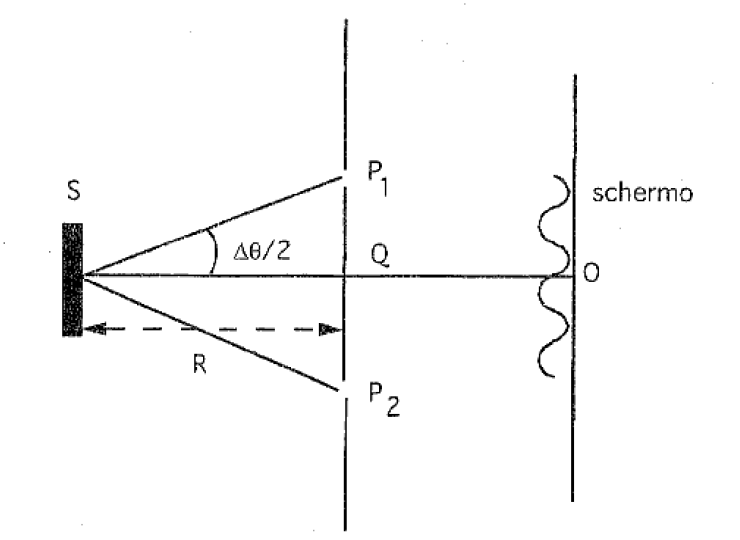
\includegraphics[width=0.6\textwidth]{Immagini/Young.png}
	\vspace{-10pt}
	\caption{}
	\label{fig:young}
	\vspace{-10pt}
\end{figure}

La presenza di frange sullo schermo è quindi è quindi una manifestazione della coerenza spaziale, infatti la capcità di due fasci di produrre frange è associata alla loro correlazione quando è introdotta una separazione spaziale, cioè quella data dalla distanza fra le sorgenti secondarie (vedi \cref{fig:young}).

Da un esperimento simile si può trovare che le frange si formano solo se la sorgente soddisfa la relazione:
\[ \Delta \theta \Delta s \leq \lambda \]
dove $ \Delta\theta $ è l'angolo sotto cui la sorgente vede le sorgenti secondarie, $ \lambda $ è la lunghezza d'onda dell'emissione. Per cui se la sorgente è a distanza $ R $ dal piano delle sorgenti secondarie le due sorgenti devono trovarsi entro un'area di ampiezza $ A_c $:
\[ A_c \simeq (R\Delta\theta_c)^2 = \frac{R^2\lambda^2}{S} \]
dove $ \Delta\theta_c $ è la quantità che satura la disuguaglianza precedente. La regione $ A_c $ è detta \textit{regione di coerenza} e la sua radice \textit{lunghezza di coerenza trasversale}. Si definisce anche l'\textit{angolo solido di coerenza}, come grandezza indipendente dalla distanza tra la sorgente e le sorgenti secondarie:
\[ \Delta\Omega = \frac{A_c}{R^2} = \frac{\lambda^2}{S} \]
C'è anche un altro angolo solido che può essere utile: quello sotteso dall'estensione della sorgente centrato nel punto medio fra le sorgenti secondarie, $ \Delta\Omega' $:
\[ S =  R^2 \Delta\Omega'\]
da cui si ottiene:
\[ A_c = \frac{\lambda^2}{\Delta\Omega'} \]

 \subparagraph{Interpretazione della coerenza spaziale} L'essenza della coerenza spaziale può essere tratta dalla seguente situazione: si immaginino due sorgenti puntiformi identiche spazialmente distanti e statisticamente indipendenti, \cref{fig:spcoh}.

\begin{figure}[h]
	\centering
	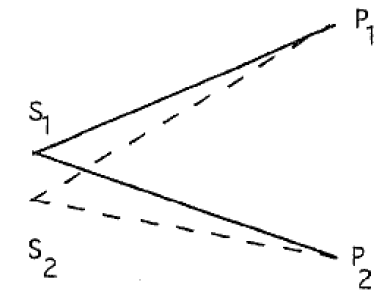
\includegraphics[width=0.4\textwidth]{Immagini/Spatialcoh.png}
	\vspace{-10pt}
	\caption{}
	\label{fig:spcoh}
	\vspace{-10pt}
\end{figure}

Si immaginino quindi due sorgenti secondarie come nel caso precedente, per le quali la differenza di cammino fra i fasci sia inferiore alla lunghezza di coerenza, $ c/\Delta\omega $, per entrambe le sorgenti. Si avrà allora che il valore dei campi prodotti nei due punti sarà lo stesso, a meno di un fattore di fase costante, dipendente dalla differenza di cammino.

Il campo totale sulle due sorgenti secondarie sarà la somma di due contributi statisticamente indipendenti. I due valori ottenuti, uno per sorgente secondaria, sono fortemente correlati: i singoli addendi differiscono solo per un termine di fase costante. In questo modo se anche le sorgenti primarie erano statisticamente indipendenti, quelle secondarie non lo sono affatto, e formano quindi una figura di interferenza sullo schermo.

\begin{oss}[Diffrazione]
	Si noti che la formula trovata per l'angolo solido di coerenza coincide con quella ottenuta per caratterizzare l'angolo solido di emissione di una sorgente diffrattiva secondaria di estensione $ S $, realizzata forando una parete opaca\footnote{Il contenuto di questa frase è che sostanzialmente non è interessante se la sorgente sia primaria o secondaria, a patto che nel secondo caso la radiazione incidente sia coerente (tipo onda piana)}.
	
	Perciò l'area di coerenza introdotta è una quantità che caratterizza i fenomeni diffrattivi dovuti all'estensione finita della sorgente.
\end{oss}

\begin{es}
	Si riportano alcuni esempi di aree di coerenza, sono omessi i calcoli.
	\begin{itemize}
		\item Sorgente d'onda termica con radiazione centrata a $ \lambda = \unit{500}{\nano\meter} $ e dimensione trasversale $ \Delta s = \unit{1}{\milli\meter} $. Per uno schermo a distanza $ R = \unit{2}{\meter} $ si ottiene $ A_c = \unit{1}{\milli\meter^2} $.
		\item Sole, con radiazione filtrata a $ \lambda = \unit{500}{\nano\meter} $. Si ottiene $ A_c \simeq \unit{3.7 \cdot 10^{-3}}{\milli\meter^2} $.
		\item Betelgeuse ($ \alpha $ di Orione), con radiazione filtrata a $ \lambda = \unit{500}{\nano\meter} $. Si ottiene $ A_c \simeq \unit{6}{\meter^2} $.
	\end{itemize}
\end{es}

Il prodotto tra l'area di coerenza $ A_c $ e la lunghezza di coerenza $ l_c $ determina un \textit{volume di coerenza}:
\[ V_c = A_c l_c = R^2 \frac{\lambda^2}{S} c \tau_c\]
e si può interpretare come la regione dello spazio in cui i fotoni sono indistinguibili gli uni dagli altri.

\subsubsection{Conteggio degli stati}

Si consideri ancora la sorgente descritta nell'esperienza di Young. Per il calcolo degli stati di singola particella si applica il procedimento descritto in \cref{sec:sumasint}: si calcola il volume di spazio delle fasi unitario e si divide per il volume della cella unitaria.

Il numero di stati è quindi:
\[ g = \frac{\Delta\Omega V p^2 \Delta p}{\hplanck^3} \]
in cui si è considerata una distribuzione isotropa in impulsi, e si selezionata la frazione a energia fissata, racchiusa nell'angolo solido di osservazione, mentre il volume $ V $ è dato dal volume occupato dai fotoni ricevuti nel tempo $ T $ di misura:
\[ V = S c T \]
L'impulso si trova a partire dall'energia dei singoli fotoni e dalla legge di dispersione:
\[ p = \frac{E}{c} = \frac{\hplanck\nu}{c} = \frac{\hbar \omega}{c} \]
Si ottiene quindi:
\[ g = \frac{\Delta\Omega S}{\lambda^2} \frac{T}{\tau_c} \]

\begin{defn}[Estensione del fascio]
	Si definisce \textit{estensione} di un fascio luminoso la quantità:
	\begin{equation*}
	U = \Delta\Omega S
	\end{equation*}
\end{defn}
La definizione di $ U $ è importante perché questa grandezza mantiene un valore costante nella propagazione di un fascio luminoso sotto le leggi dell'ottica geometrica.

Per il caso dell'angolo solido $ \Delta\Omega $ determinato dalla diffrazione della superficie $ S $ della sorgente si ottiene che l'estensione ha il valore $ U_c $:
\[ U_c = \frac{\lambda^2}{S} S = \lambda^2 \]
e quindi il numero degli stati è:
\[ g = \frac{U}{U_c} \frac{T}{\tau_c} \]
in cui il primo termine è definito \textit{fattore di coerenza spaziale} e il secondo \textit{fattore di coerenza temporale}.

\begin{oss}
	Il fattore di coerenza spaziale può essere scritto nella forma:
	\[ \frac{U}{U_c} = \frac{S'}{A_c} \]
	con $ S' = R^2 \Delta\Omega $ cioè l'area di osservazione. In questa forma tale fattore diventa analogo al fattore di coerenza temporale, cioè il rapporto tra una grandezza relativa all'osservazione e una grandezza caratterizzante le proprietà di coerenza della sorgente.
\end{oss}

Poiché $ g $ corrisponde a un numero intero, il cui minimo è $ 1 $, si ha che i due fattori di coerenza non possono mai essere minori di $ 1 $ individualmente (se uno dei due lo fosse si potrebbe portare a $ 1 $ l'altro riducendo $ g $ a un valore inferiore all'unità), per cui non possono essere utilizzati per compensarsi a vicenda.

Se i valori delle grandezze di osservazione sono maggiori di quelli delle grandezze di coerenza si otterrà una figura a contrasto più basso, perché i fotoni raccolti non sono tutti coerenti fra loro.

\begin{es}[Numero di stati]
	Il valore dell'\textit{estensione di coerenza} è determinato dalla sola lunghezza d'onda della radiazione raccolta. Considerando il valore degli esempi precedenti, $ \lambda = \unit{500}{\nano\meter} $, si ha $ U_c = \unit{25\cdot10^{-10}}{\centi\meter^2}$. Per una sorgente di $ S = 1 \milli\meter^2 $ posta a distanza $ R = 1 \meter $ da uno schermo di $ S' = 1 \centi\meter^2 $ si ottiene:
	\[ \frac{U}{U_c} = 400 \]
	Per cui bisognerebbe porsi molto più lontano per diminuire questo numero (infatti se lo schermo fosse più lontano diminuirebbe l'angolo solido sotteso). Per un valore pari a $ 1 $ per il fattore di coerenza occorrerebbe porsi a $ 20 \meter $ di distanza.
	
	\noindent La parte temporale è stata già discussa, infatti il periodo di osservazione andrà adeguato al tempo di coerenza $ \tau_c $.
\end{es}

\subsection{Interferometria stellare e di Hanbury Brown e Twiss}

L'interferometro di Hanbury Brown e Twiss è un'evoluzione dell'interferometro stellare di Michelson. Esso è stato usato per la misura dei \textit{raggi angolari} delle stelle viste dalla Terra.

\begin{figure}[b]
	\centering
	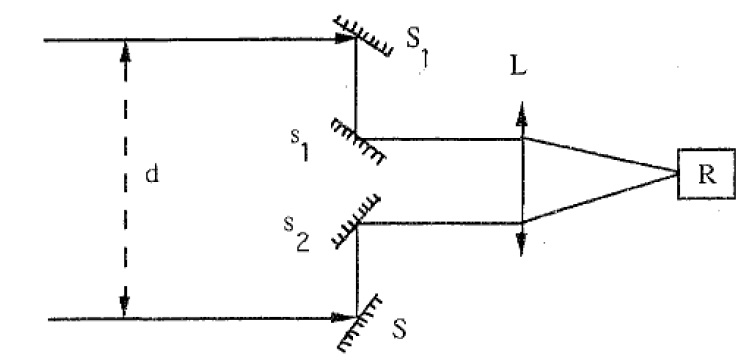
\includegraphics[width=0.6\textwidth]{Immagini/StellarMichelson.png}
	\vspace{-10pt}
	\caption{}
	\label{fig:michelsonst}
	\vspace{-10pt}
\end{figure}

\paragraph{Interferometro stellare di Michelson} Nell'interferometro di Michelson, \cref{fig:michelsonst}, la luce di una sorgente distante (una stella) arriva su due specchi primari $ S_1$ ed $ S_2 $, separati da una disanza $ d $ che può essere variata. La luce viene riflessa su due specchi secondari $ s_1$ ed $ s_2 $ e convogliata attraverso una lente $ L $ su  un rivelatore.

Finché i due specchi primari sono distanti meno di una lunghezza di coerenza trasversale (cioè appartengono alla stessa area di coerenza) il contrasto della figura di interferenza dipende solo dal fattore temporale. La condizione è quindi:
\[ d < \sqrt{A_c} = \frac{2}{\sqrt{\pi}}\frac{R \lambda}{a} = \frac{2}{\sqrt{\pi}}\frac{\lambda}{\alpha} \]
dove si è espressa l'area $ S $ della stella attraverso il suo diametro $ a $:
\[ S = \frac{\pi a^2}{4} \]
e il diametro angolare $ \alpha $ attraverso la distanza dalla Terra $ R $:
\[ \alpha = \frac{a}{R} \]
perciò testando la disuguaglianza per $ d $ si può misurare $ \alpha $.

\paragraph{Interferometro di Hanbury Brown e Twiss} Nel metodo di Hanbury Brown e Twiss si sostituiscono le due coppie di specchi (destra e sinistra) con due rivelatori, che forniscono dei segnali elettrici associati all'intensità luminosa (vedi \cref{fig:hbrowntwiss}).

\begin{figure}[t]
	\centering
	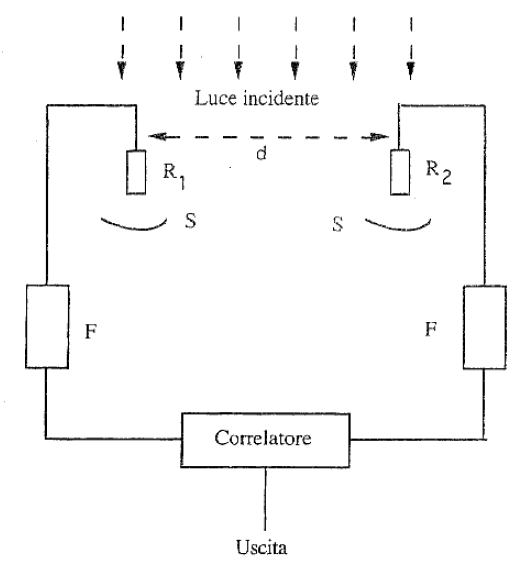
\includegraphics[width=0.6\textwidth]{Immagini/HanburyBrownTwiss.png}
	\vspace{-10pt}
	\caption{}
	\label{fig:hbrowntwiss}
	\vspace{-10pt}
\end{figure}

I segnali elettrici presentano fluttuazioni, che vengono esaminate attraverso il \textit{correlatore}. La misura si ottiene come nel caso di MIichelson variando la distanza $ d $ e misurando le correlazioni.

Siano quindi $ N_1, N_2 $ il numero dei fotoni che arrivano sui due rivelatori, e $ \overline{N_1}, \overline{N_2} $ i rispettivi valori medi. Il segnale di correlazione è definito come:
\[ C = (N_1 - \overline{N_1})  (N_2 - \overline{N_2}) \]
ed il correlatore fornisce la media di questa quantità, $ \overline{C} $. Se i rivelatori sono nella stessa area di coerenza (come nel caso di Michelson) il numero di possibili stati di singola particella è quindi $ g = T/\tau_c $, perché il fattore di coerenza spaziale è unitario.

Come descritto nella \cref{sec:fotonfluct}, questa volta però considerando anche il contributo corpuscolare, si ottiene per le fluttuazioni:
\[ \overline{(N_1 - \overline{N_1})^2} = \overline{N_1} + \frac{\overline{N_1}^2}{g} \]
e la stessa cosa si ottiene anche per $ N_2 $ e $ N = N_1 + N_2 $.

Esplicitando la relazione per $ N $ in termini di $ N_1,N_2 $ si ottiene:
\begin{align*}
\overline{(N_1 + N_2 - \overline{N_1 + N_2})^2} = \overline{N_1 + N_2} &+ \frac{\overline{N_1 + N_2}^2}{g}\\
\overline{(N_1 - \overline{N_1})^2} + \overline{(N_2 - \overline{N_2})^2} + 2 \overline{(N_1 - \overline{N_1})(N_2 - \overline{N_2})}& = \overline{N_1} + \frac{\overline{N_1}^2}{g} + \overline{N_2} + \frac{\overline{N_2}^2}{g} + 2 \frac{\overline{N_1}\overline{N_2}}{g}
\end{align*}
da cui, eliminando le relazioni trovate sopra per $ N_1, N_2 $, si ottiene l'espressione per la correlazione mediata sul tempo:
\[ \overline{C} = \overline{(N_1 - \overline{N_1})  (N_2 - \overline{N_2})} = \frac{\overline{N_1}\overline{N_2}}{g} \]

Quando i rivelatori vengono allontanati e la loro distanza supera la lunghezza trasversale di coerenza la formula per la correlazione media non è più valida, si può affermare però che essa diminuisce rapidamente.

\begin{oss}[Altre statistiche]
	La formula trovata vale per particelle che obbediscono alla statistica di Bose, per trovare l'espressione nel caso delle statistiche di Fermi e di Boltzmann è sufficiente modificare l'espressione per $ \overline{(N_1 - \overline{N_1})^2} $: nel primo caso al secondo membro il termine ondulatorio ha un segno meno, mentre nel caso classico è del tutto assente.
	
	Questo porta ad un segno $ - $ nella correlazione media dei fermioni, rispetto a quella dei bosoni, mentre porta ad annullarsi completamente la correlazione nel caso di particelle classiche.
\end{oss}

Per bosoni e fermioni il comportamento della correlazione media può essere spiegato in termine dei fenomeni di bunching e anti-bunching introdotto nella \cref{sec:fotonfluct}:
\begin{itemize}
	\item i bosoni tendono a raccogliersi insieme, per cui un aumento del numero di fotoni su un rivelatore indica un \textit{bunch} con più fotoni, per cui è probabile trovare più fotoni anche sull'altro;
	\item ai fermioni, a causa del principio di esclusione di Pauli, è proibito viaggiare insieme, per cui a un aumento dei fotoni su un rivelatore corrisponderà una diminuzione sull'altro.
\end{itemize}
I comportamenti discussi si possono anche pensare alla luce delle interazioni efficaci fra particelle quantistiche introdotte nella \cref{sec:fewdegas}.
\newline

Il vantaggio di questo esperimento rispetto a quello di Michelson è che impiegano i due rivelatori anziché uno solo si elimina il termine classico delle fluttuazioni e si misura solo quello quantistico.

Poiché cioè che si misura è il prodotto delle intensità sui due rivelatori l'uscita dipende dalla quarta potenza del campo elettrico.

\paragraph{Misura della coerenza temporale} Nella descrizione dell'esperimento si è detto che viene variata la distanza $ d $ al fine di trovare la coerenza spaziale del segnale (lunghezza di coerenza trasversale).
Si può però scegliere di tenere fissa la distanza $ d $, all'interno dell'area di coerenza, e introdurre un ritardo temporale all'uscita di uno dei due rivelatori, e misurare la coerenza temporale:
\[ \overline{C(\tau)} = \overline{(N_1(t) - \overline{N_1})  (N_2(t+\tau) - \overline{N_2})} \]

Si osserverà quindi una forte correlazione per ritardi $ \tau < \tau_c $, mentre la correlazione diminuirà quando il ritardo sarà maggiore del tempo di coerenza.

\`E quindi possibile caratterizzare in maniera completa le proprietà di coerenza della radiazione incidente.

\section{Rumore}

\subsection{Teorema di Nyquist}

Nel $ 1927 $ Johnson ha osservato che ai capi di un elemento generico di un circuito elettrico (tipicamente il più semplice: una resistenza) sono presenti della fluttuazioni nel segnale dovute alla temperatura finita del componente. Tali fluttuazioni sono perciò definite \textit{rumore termico} o \textit{Johnson}.
La spiegazione fu immediatamente fornita Nyquist, da cui il risultato teorico noto come \textit{teorema di Nyquist}.
\newline

L'enunciato del teorema è il seguente: si consideri una resistenza $ R $ alla temperatura $ T $, ai suoi capi verrà generata una tensione fluttuante che se misurata in una banda di frequenza $ \Delta f $ possiede un valore quadratico medio:
\[ \overline{V_{\Delta f}^2} = 4 R \kt \Delta f \]

Il teorema di Nyquist ha due importanti caratteristiche:
\begin{itemize}
	\item è valido per ogni circuito elettronico;
	\item è un primo esempio del teorema di fluttuazione-dissipazione: lega l'ampiezza delle fluttuazione all'elemento dissipativo $ R $ del sistema.
\end{itemize}

\begin{oss}[Dipendenza dalla banda passante]
	La dipendenza dell'ampiezza delle fluttuazioni dalla banda passante ha una motivazione evidente: una banda passante minore implica l'integrazione del segnale per tempi più lunghi. Se il segnale è a media nulla queste fluttuazioni saranno sempre più attenuate per tempi di integrazione sempre maggiori, poiché le fluttuazioni positive compenseranno quelle negative (per alte bande passanti il problema non si pone nemmeno: le alte frequenze sono fortemente smorzate dagli elementi capacitivi, per cui sono segnali deboli e soggetti ad ogni sorta di rumore).
\end{oss}

Si consideri una linea di trasmissione senza perdita di lunghezza $ l $ ed impedenza caratteristica $ R $, terminata da entrambi i lati da una resistenza di carico $ R $.
Tutti gli elementi sono a contatto con un bagno termico, che fissa la loro temperatura a $ T $. La situazione è schematizzata in \cref{fig:nyqline}.

\begin{figure}[b]
	\centering
	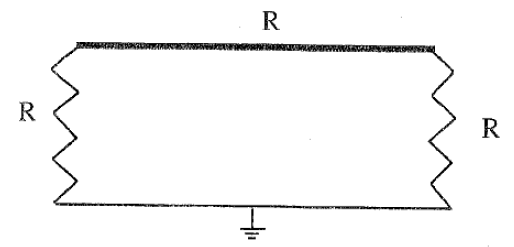
\includegraphics[width=0.6\textwidth]{Immagini/NyquistLine.png}
	\vspace{-10pt}
	\caption{}
	\label{fig:nyqline}
	\vspace{-10pt}
\end{figure}

Se si considera la propagazione di onde elettromagnetiche di lunghezza $ \lambda $ lungo tutta la linea. La linea presenta risonanze se:
\[ l = n \frac{\lambda}{2} \qquad \text{con}~n \in \mathbb{N} \]
Se $ c' $ è la velocità di propagazione lungo la linea si ha:
\[ l = n \frac{c'}{2 \nu} \implies n = l \frac{2\nu}{c'} \]
per cui in un intervallo di frequenza $ \Delta \nu $ ci saranno $ 2l \Delta \nu /c' $ modi di vibrazione.
Secondo la statistica di Bose ad ogni modo è associata un'energia:
\[ h\nu \bar{n} = h \nu \frac{1}{\exp[\frac{h\nu}{\kt}] - 1} \]
e nel limite classico $ h\nu \ll \kt $ l'energia diventa proprio $ \kt $. L'energia associata alla linea quindi risulta:
\[ h\nu \bar{n} \frac{2l}{c'} \Delta f \simeq \kt \frac{2l}{c'} \Delta f \]
e l'energia che si propaga per ogni direzione è la metà.

Questa energia viene portata alla resistenza in un tempo $ l/c' $, per cui la potenza per unità di tempo dissipata a carico della resistenza è:
\[ P_{\Delta f} = \kt \Delta f \]
Poiché si è all'equilibrio anche il carico $ R $ emette energia allo stesso ritmo, per cui la resistenza stessa genera alla temperatura $ T $ una potenza $ P_{\Delta f} $.

\begin{figure}[t]
	\centering
	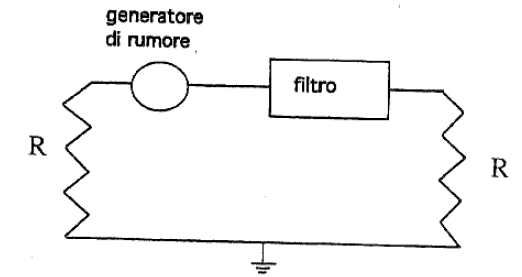
\includegraphics[width=0.6\textwidth]{Immagini/NyquistNoiseGenerator.png}
	\vspace{-5pt}
	\caption{}
	\label{fig:nyqgen}
	\vspace{-10pt}
\end{figure}

Il sistema può essere schematizzato sostituendo la linea di trasmissione con un generatore di rumore e un filtro per la banda di frequenza d'interesse, come mostrato in \cref{fig:nyqgen}.

Nella resistenza di carico scorre quindi una corrente $ I_{\Delta f} $ tale che la potenza sia quella prodotta dalla linea, cioè:
\[ I_{\Delta f}^2 R = \kt \Delta f \]
allora il generatore di rumore è un generatore di tensione $ V_{\Delta f} $ con:
\[ V_{\Delta f} = 2 R I_{\Delta f} \]
% non capisco perché il 2
e quindi:
\[ V_{\Delta f}^2 = 4 R \kt \Delta f \]
che è esattamente la tesi del teorema di Nyquist.

\paragraph{Generalizzazione ad impedenze complesse} Il teorema può essere generalizzato per impedenze complesse, semplicemente considerando un circuito costituito da tre elementi in serie: una resistenza $ R $, un'impedenza complessa $ Z = X + i Y $ e un filtro, che selezioni la banda d'interesse.

Sia $ \overline{V_{\Delta f}^2(R)} $ il quadrato della tensione di rumore prodotta da $ R $ in una banda di frequenza $ \Delta f $. La potenza dissipata in $ Z $ sarà:
\[ P_Z = \overline{\Re\{IZ\} \Re\{I\}} = \frac{1}{2} \Re\{(IZ) I^\ast\} = \frac{1}{2} ((IZ) I^\ast + (IZ)^\ast I) = \frac{1}{2}\abs{I}^2 (Z + Z^\ast) = \frac{\overline{V_{\Delta f}^2(R)}}{(R+X)^2 + Y^2}X\]
dove si è usato che:
\[ I = \frac{\overline{V_{\Delta f}^2(R)}}{R + X +iY} \]

Viceversa associando una tensione $ V_{\Delta f}(Z) $ di rumore all'impedenza $ Z $ si scrive la potenza dissipata in $ R $ come:
\[  P_R = \frac{\overline{V_{\Delta f}^2(Z)}}{(R+X)^2 + Y^2}R \]

Essendo all'equilibrio le due potenza scritte sopra devono essere uguali, per cui:
\[ \overline{V_{\Delta f}^2(Z)} R = \overline{V_{\Delta f}^2(R)} X \]
da cui si ricava facilmente il valore per $ \overline{V_{\Delta f}^2(Z)} $:
\[ V_{\Delta f}^2(Z) = 4 X \kt \Delta f\]

\begin{es}
	Per una temperatura pari a $ 293 \kelvin $, una banda di frequenza $ 1 \hertz $ e una resistenza di carico di $ 1 \mega\ohm $ si ottiene:
	\[ \sqrt{V_{\Delta f = 1}^2} = 0.127 \micro\volt \]
\end{es}

\subsection{Teorema di Wiener-Khintchine}

\subsection{Derivazione microscopica del Teorema di Nyquist}

\subsection{Shot noise}